\documentclass[14pt]{report}
\usepackage[a4paper, total={6.5in, 10.5in}]{geometry}
\usepackage{amsmath,amsfonts,amsthm,amssymb}
\usepackage{fancyhdr}
\usepackage{color}
\usepackage{graphicx}
\usepackage{subcaption}
\usepackage{enumerate}

% Set the section numbering to 1, 2, 3, and so on.
\renewcommand\thesection{\arabic{section}}

% Report front page.
\title{Automating Roll Calls with Deep Metric Learning}
\author{Guan-Zhong Wang (U10516045)\\[1cm]{Supervisor: Chun-Ming Tsai}}
\begin{document}
\maketitle
\date

% Report content.
\begin{center}
  \section*{\abstractname}
\end{center}
\large

In my semester project, I prototyped a roll call system called \textbf{pyRollCall} in Python 3.5 to automate 
the traditional roll call procedures with deep metric learning.
\newline

Normally, a teacher needs to call each student's name one by one in order to check who is present
at a class. This system aims to simplify the traditional roll call procedures by pre-computing each 
student's facial embeddings using \textbf{dlib}, so that it can identify students' faces correctly later
with \textbf{OpenCV} as well as \textbf{face\_recognition} module and completely automates roll calls.
\newline


\section{Introduction}
With the rapid growth of technology, more and more repetitive tasks can be automated by programs.
In my semester project, I built a system to replace the tedious procedure of a traditional roll call.
\newline

Initially, the users (typically teachers) are required to populate the database with the information
of the courses and students he/her teaches. Secondly, the users have to take several photos of each
student presented in the database and compute their facial embeddings. Lastly, the program can start
identifying students' faces and help users automate roll calls.
\newline

\section{Implementation}
This system employs a technique called \textbf{deep metric learning} (i.e., deep-learning-based facial recognition)
to quantify the faces of students via dlib and face\_recognition module. In order to achieve facial 
recognition in Python and OpenCV, I referenced the tutorial [1] on pyimagesearch by Adrian Rosebrock.
\newline

According to the tutorial [1], the network architecture for face recognition being used in this system 
is based on ResNet-34 from the \textit {Deep Residual Learning for Image Recognition} paper [2] by Kaiming He, 
Xiangyu Zhang, Shaoqing Ren and Jian Sun. The network in dlib was already trained by the creator of dlib,
Davis King, on a dataset of approximately three million images, while face\_recognition is a wrapper of
dlib which enables users to use it easily.
\newline

Users can manage their data, including courses, students and facial embeddings through GUI\@. They can also 
initiate a roll call through GUI, letting students sign in to a class with facial recognition, as shown in
Figure 1.
\newline

\begin{figure}[b!]
  \centering
  \begin{subfigure}[b]{0.32\linewidth}
    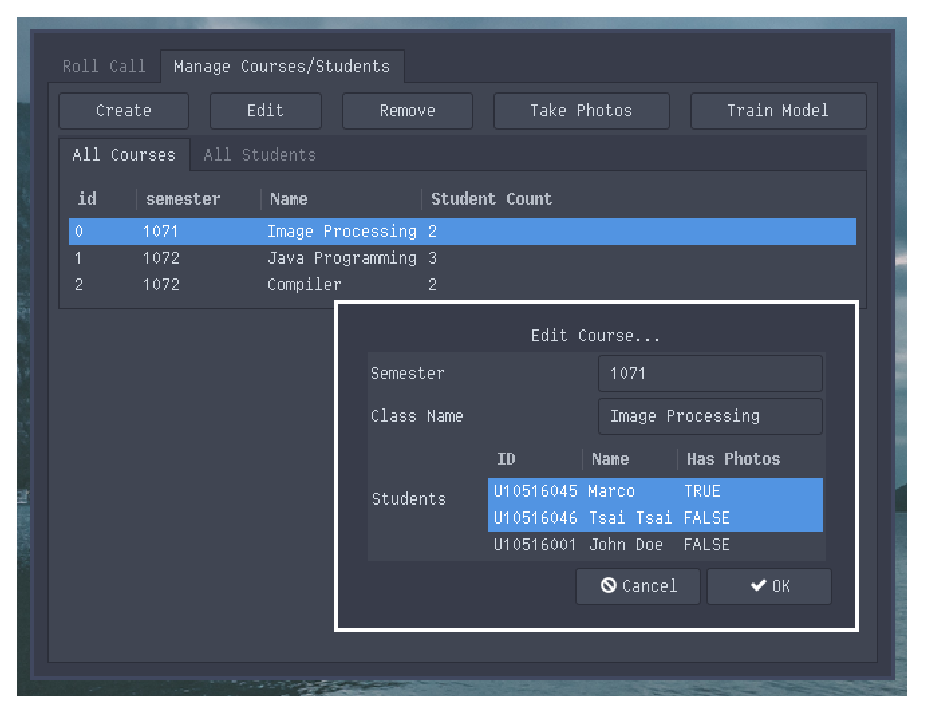
\includegraphics[width=\linewidth]{figures/preview1.eps}
    \caption{Managing courses.}
  \end{subfigure}
  \begin{subfigure}[b]{0.32\linewidth}
    
\includegraphics[width=\linewidth]{figures/preview2.eps}
    \caption{Managing students.}
  \end{subfigure}
  \begin{subfigure}[b]{0.32\linewidth}
    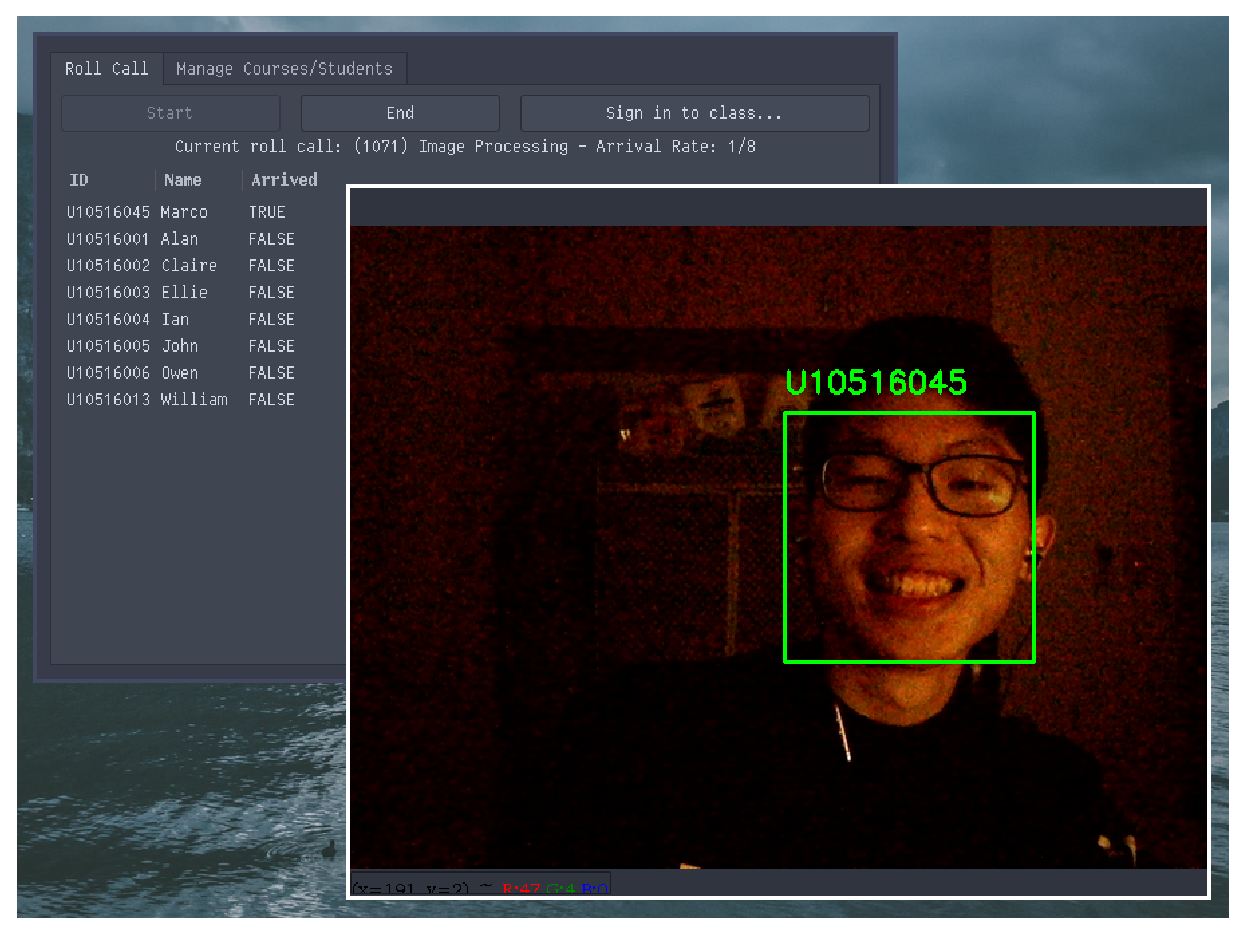
\includegraphics[width=\linewidth]{figures/preview3.eps}
    \caption{A student signing in.}
  \end{subfigure}
  \caption{pyRollCall's GUI, database and facial recognition.}
  \label{fig:implementation}
\end{figure}


\section{Experimental Results}
I experimented this system on 7 people, including 6 famous actors from the movie Jurassic Park (1993) and
myself, with each of them given a student ID (e.g., U10516001). The training image set of the 6 actors is
from the tutorial [1] on pyimagesearch.
\newline

\begin{enumerate}
  \item U10516001 - Alan Grant (22 images)
  \item U10516002 - Claire Dearing (53 images)
  \item U10516003 - Ellie Sattler (31 images)
  \item U10516004 - Ian Malcolm (41 images)
  \item U10516005 - John Hammond (36 images)
  \item U10516006 - Owen Grady (35 images)
  \item U10516045 - Guan-Zhong Wang (5 images)
\end{enumerate}

It can distinguish between 7 different people, successfully automating a roll call, as shown in Figure 2.

\begin{figure}[h!]
  \centering
  \begin{subfigure}[b]{0.32\linewidth}
    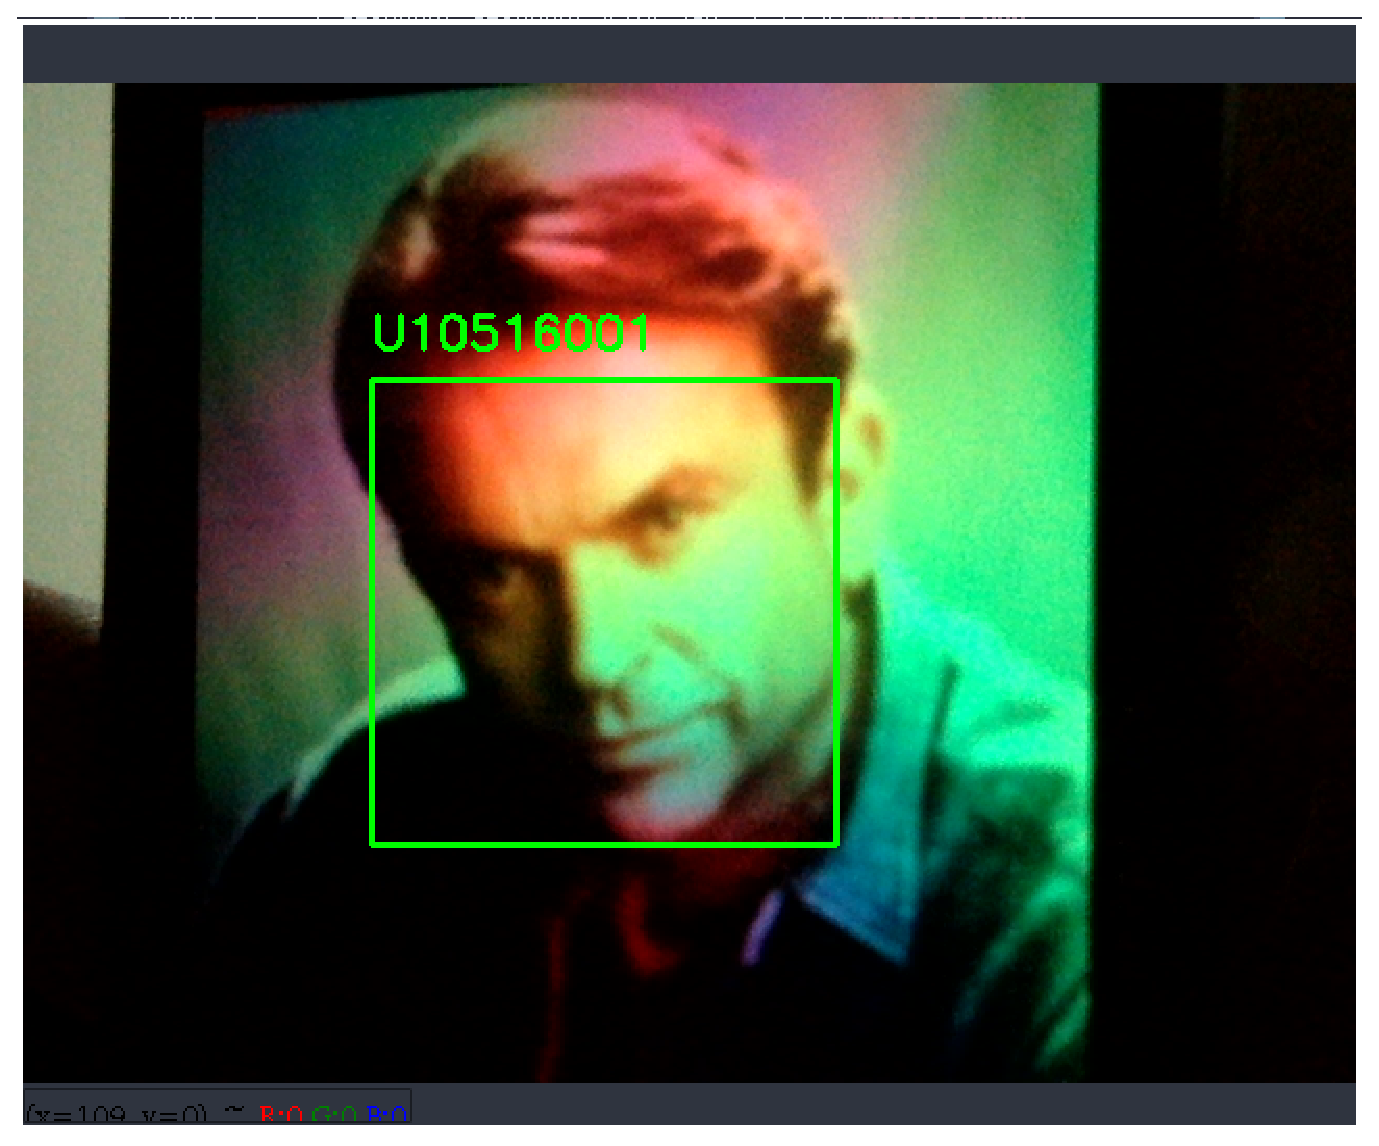
\includegraphics[width=\linewidth]{figures/exp01.eps}
    \caption{U10516001 Alan Grant.}
  \end{subfigure}
  \begin{subfigure}[b]{0.32\linewidth}
    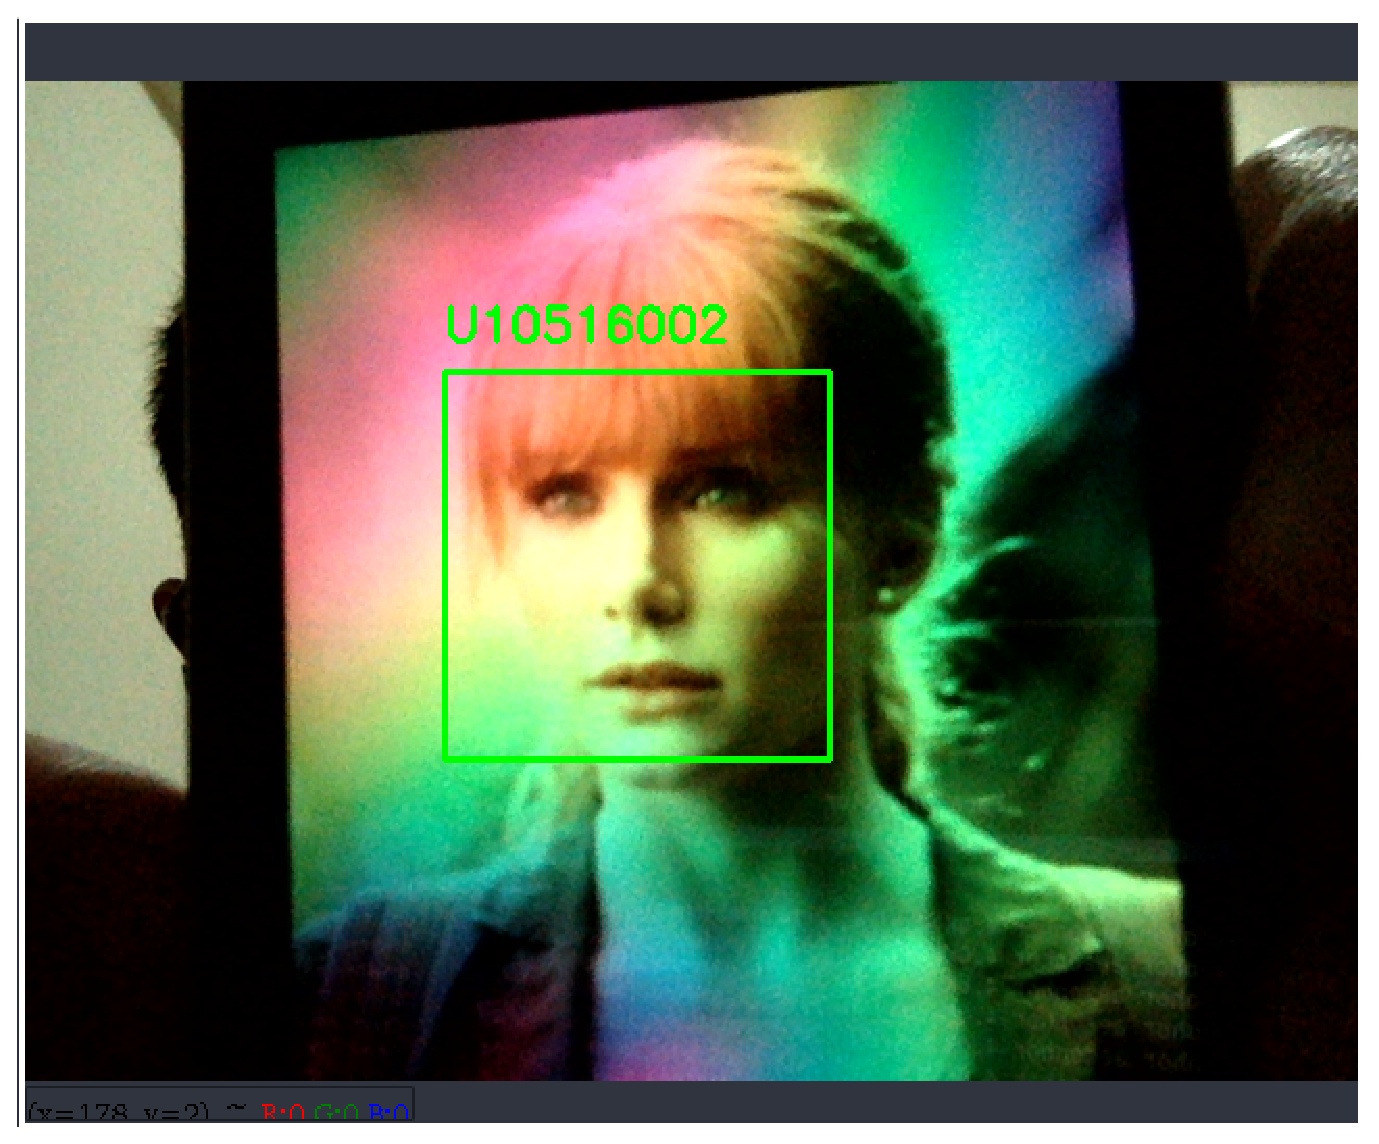
\includegraphics[width=\linewidth]{figures/exp02.eps}
    \caption{U10516002 Claire Dearing.}
  \end{subfigure}
  \begin{subfigure}[b]{0.32\linewidth}
    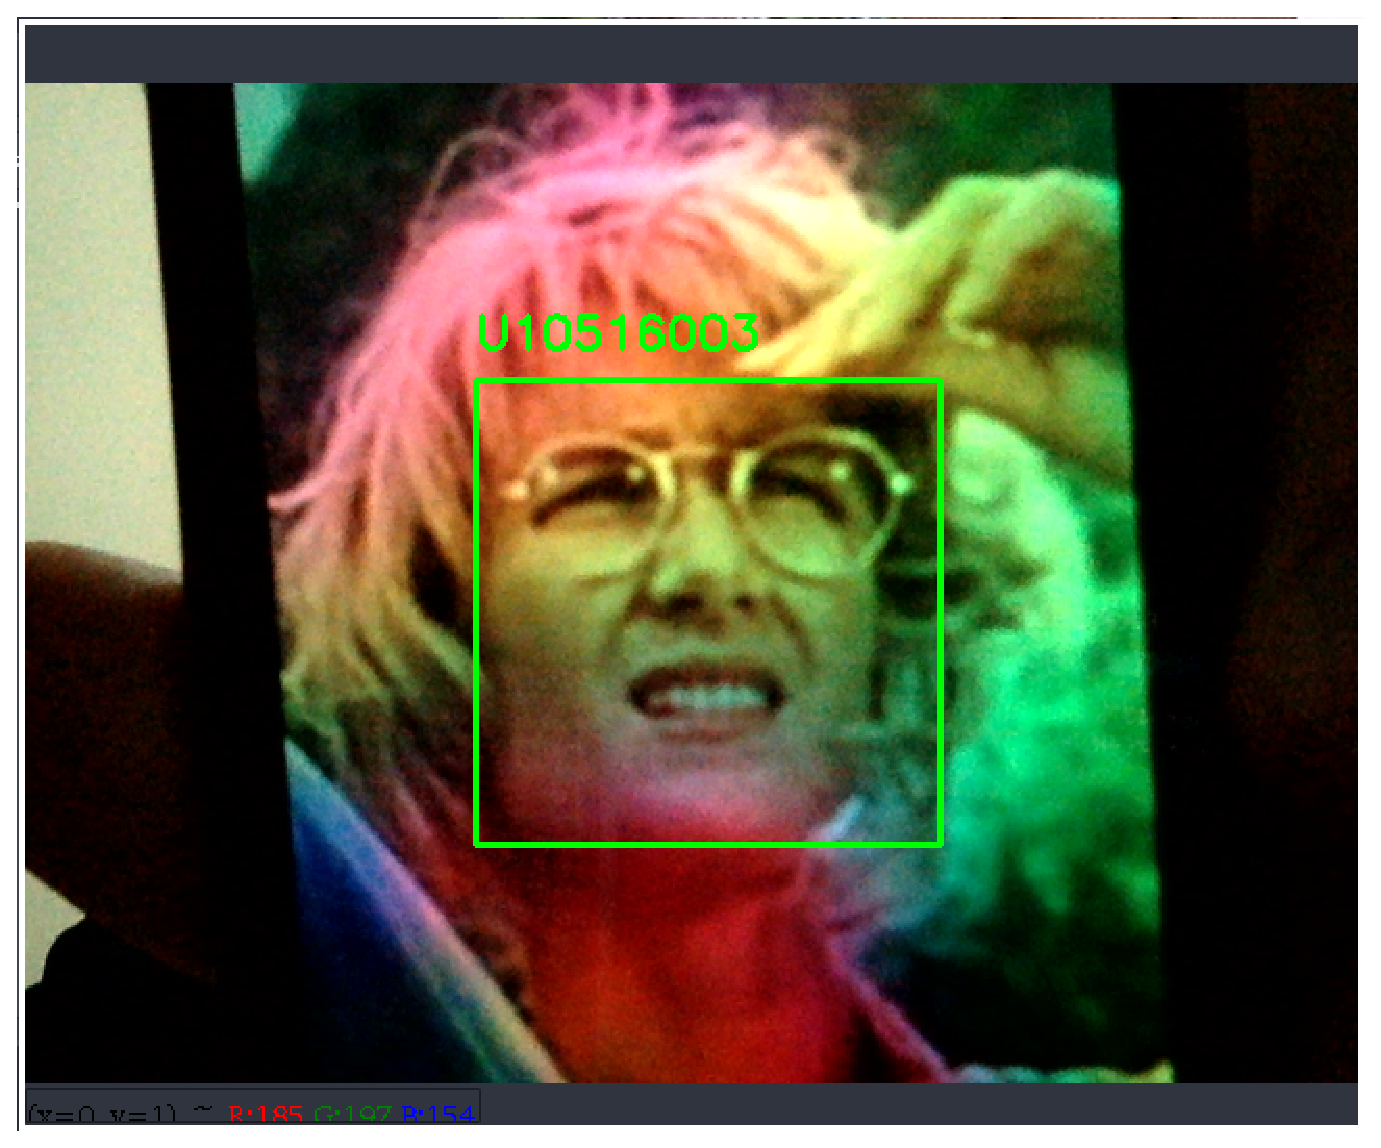
\includegraphics[width=\linewidth]{figures/exp03.eps}
    \caption{U10516003 Ellie Sattler.}
  \end{subfigure}
  \begin{subfigure}[b]{0.32\linewidth}
    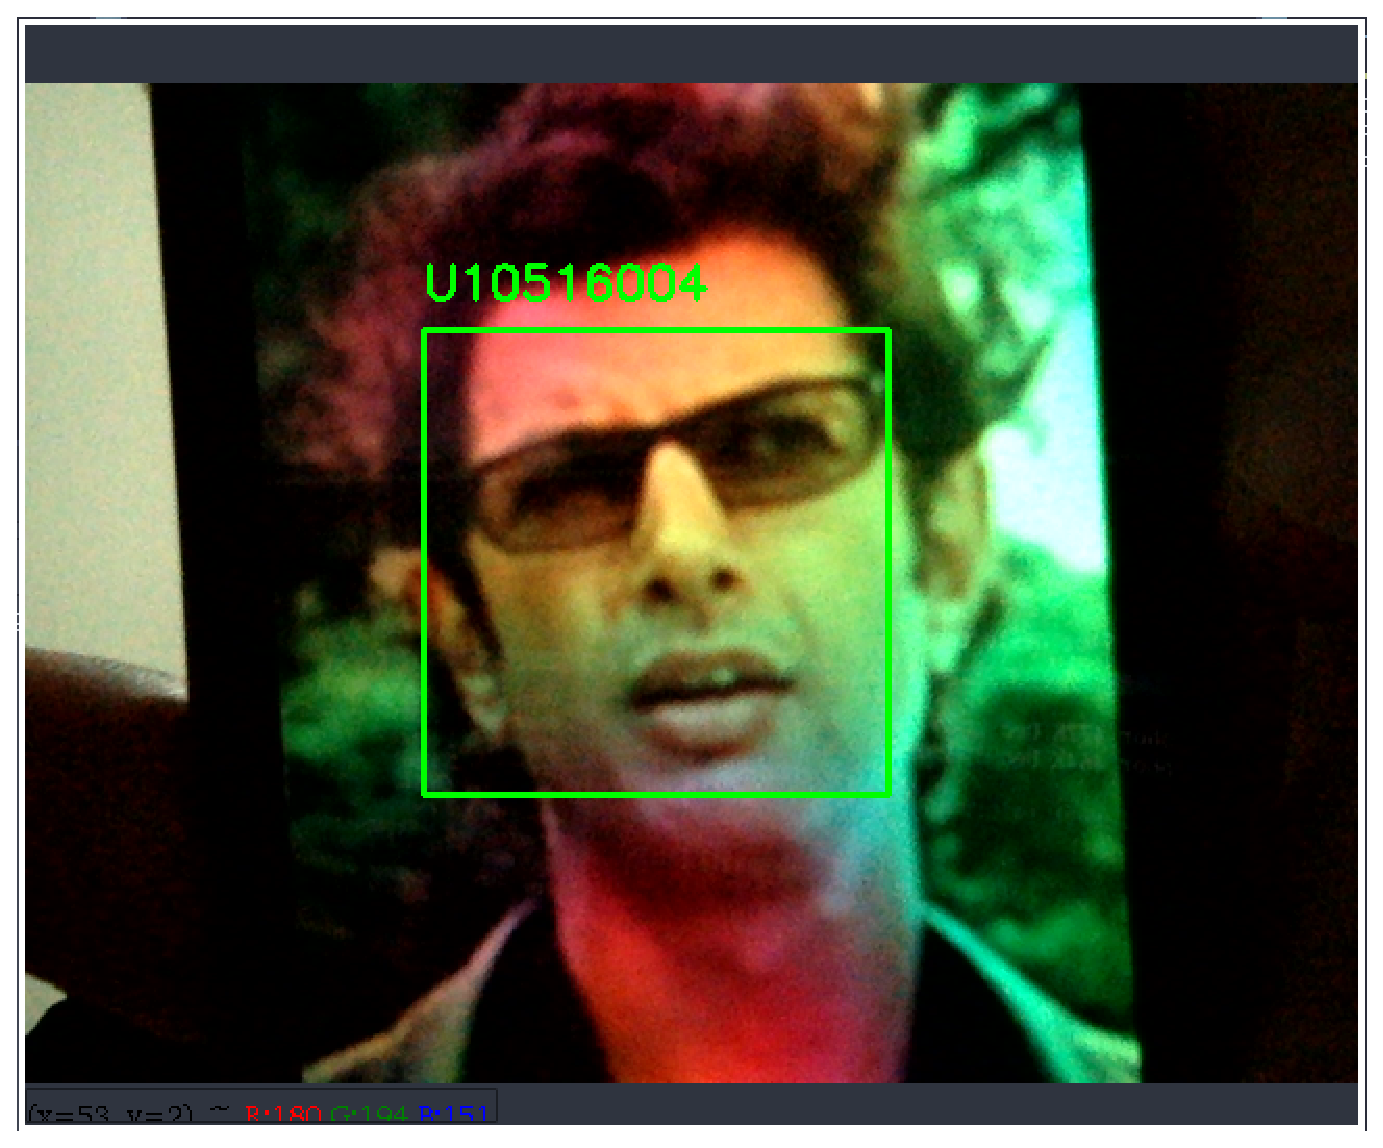
\includegraphics[width=\linewidth]{figures/exp04.eps}
    \caption{U10516004 Ian Malcolm.}
  \end{subfigure}
  \begin{subfigure}[b]{0.32\linewidth}
    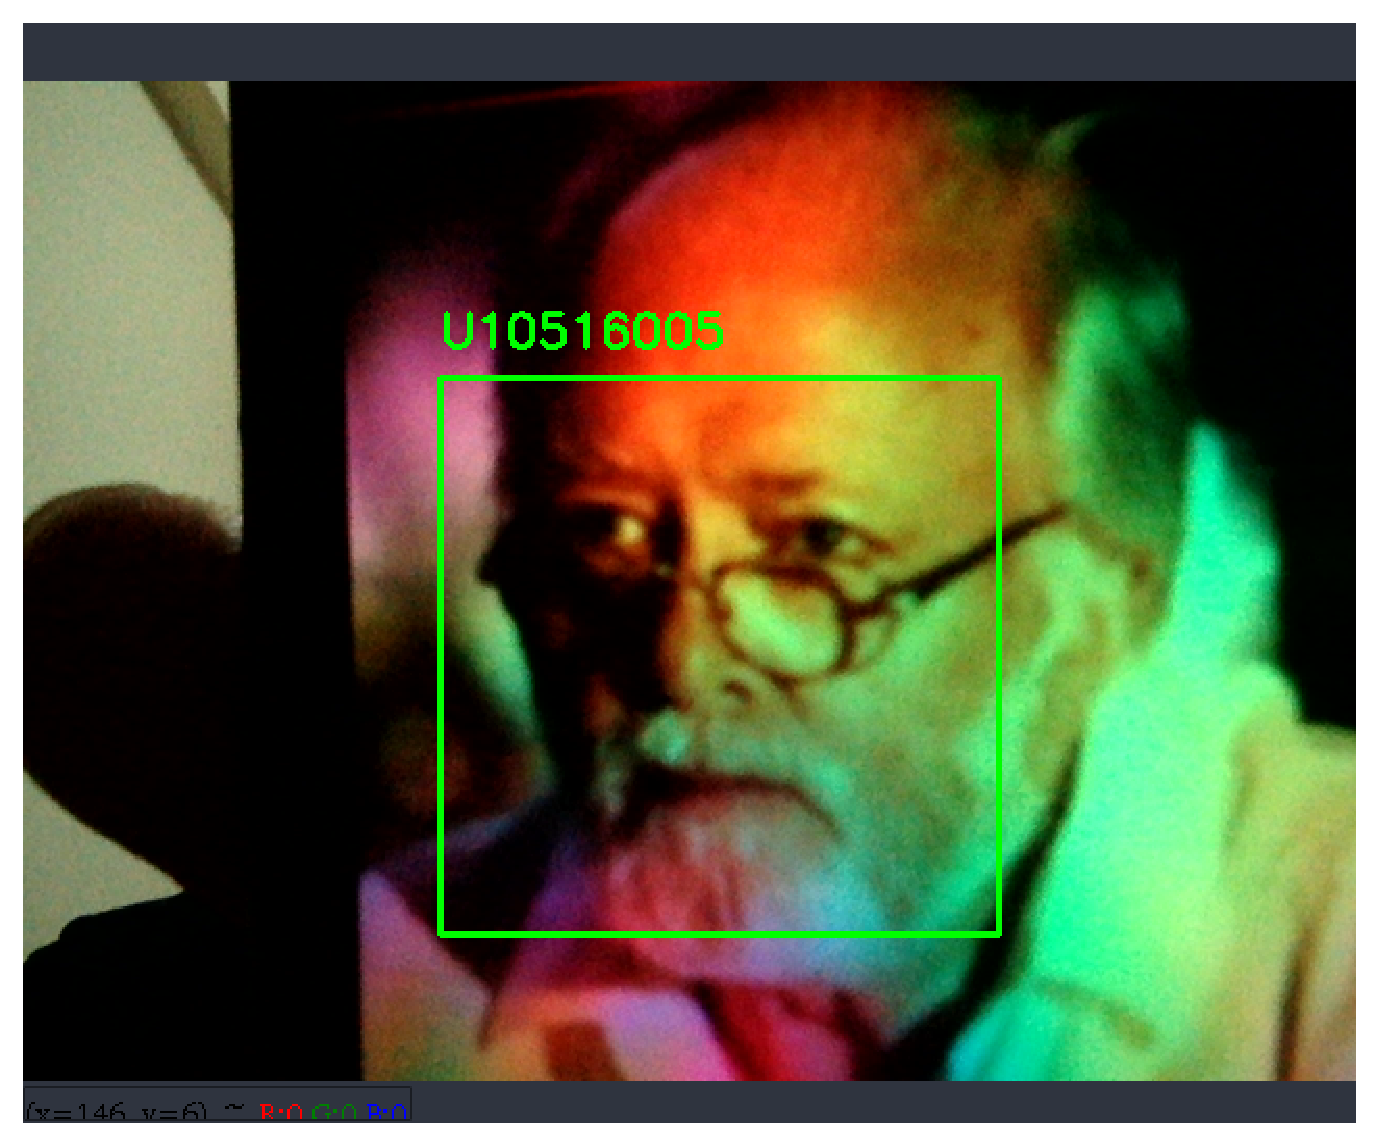
\includegraphics[width=\linewidth]{figures/exp05.eps}
    \caption{U10516005 John Hammond.}
  \end{subfigure}
  \begin{subfigure}[b]{0.32\linewidth}
    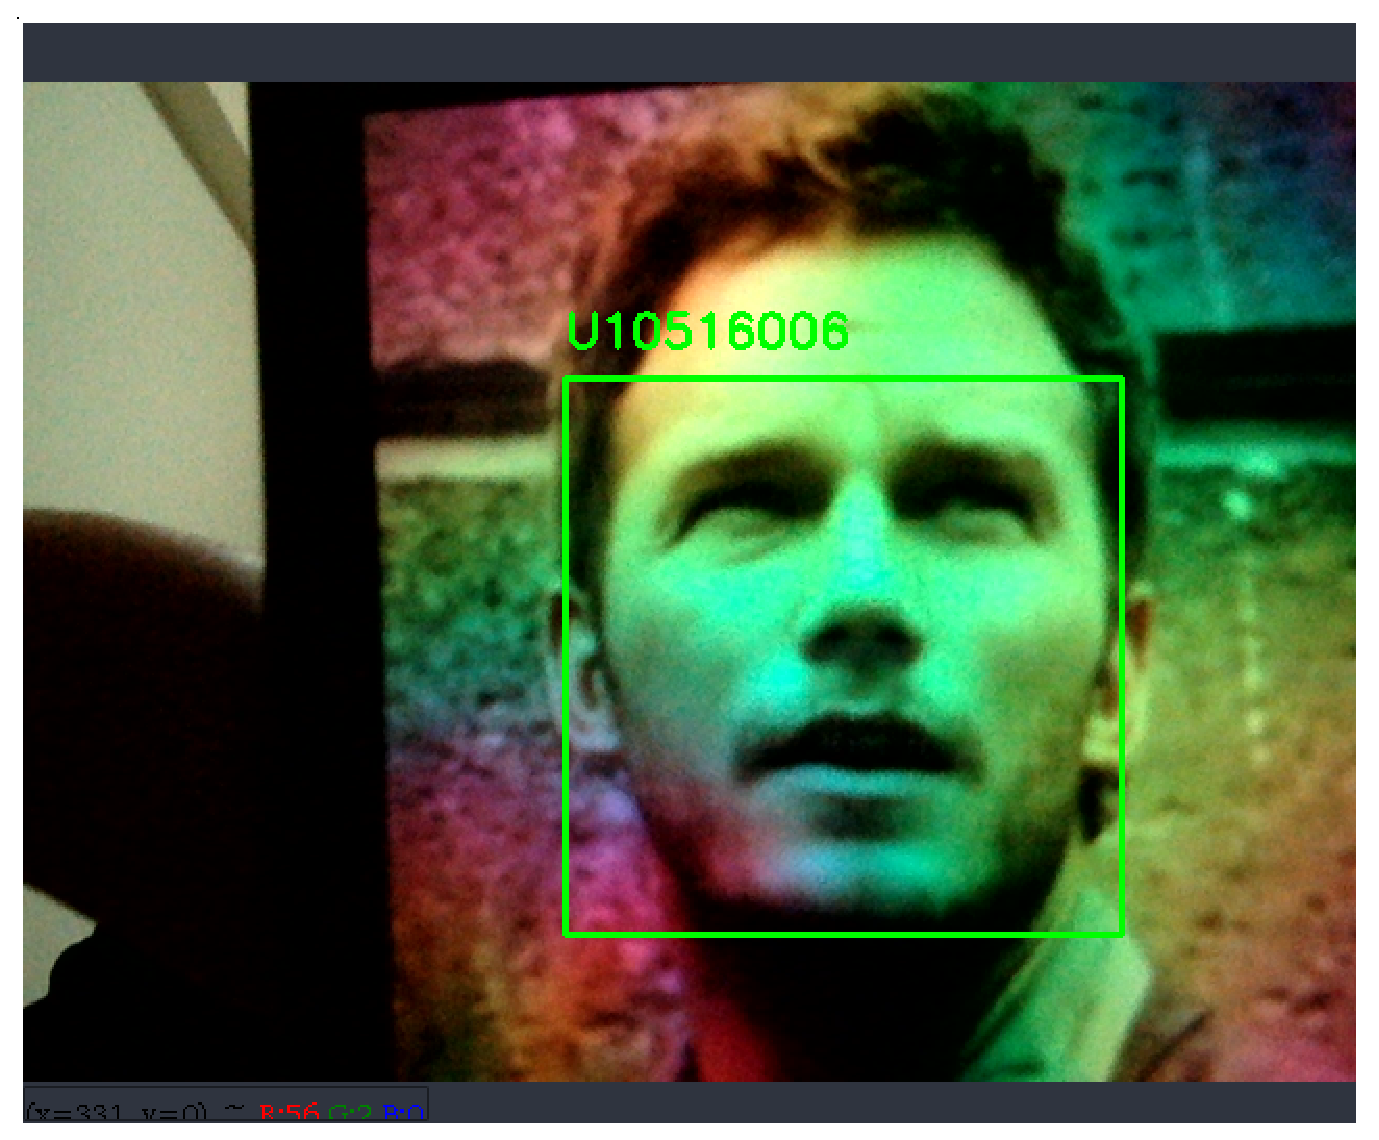
\includegraphics[width=\linewidth]{figures/exp06.eps}
    \caption{U10516006 Owen Grady.}
  \end{subfigure}
  \begin{subfigure}[b]{0.32\linewidth}
    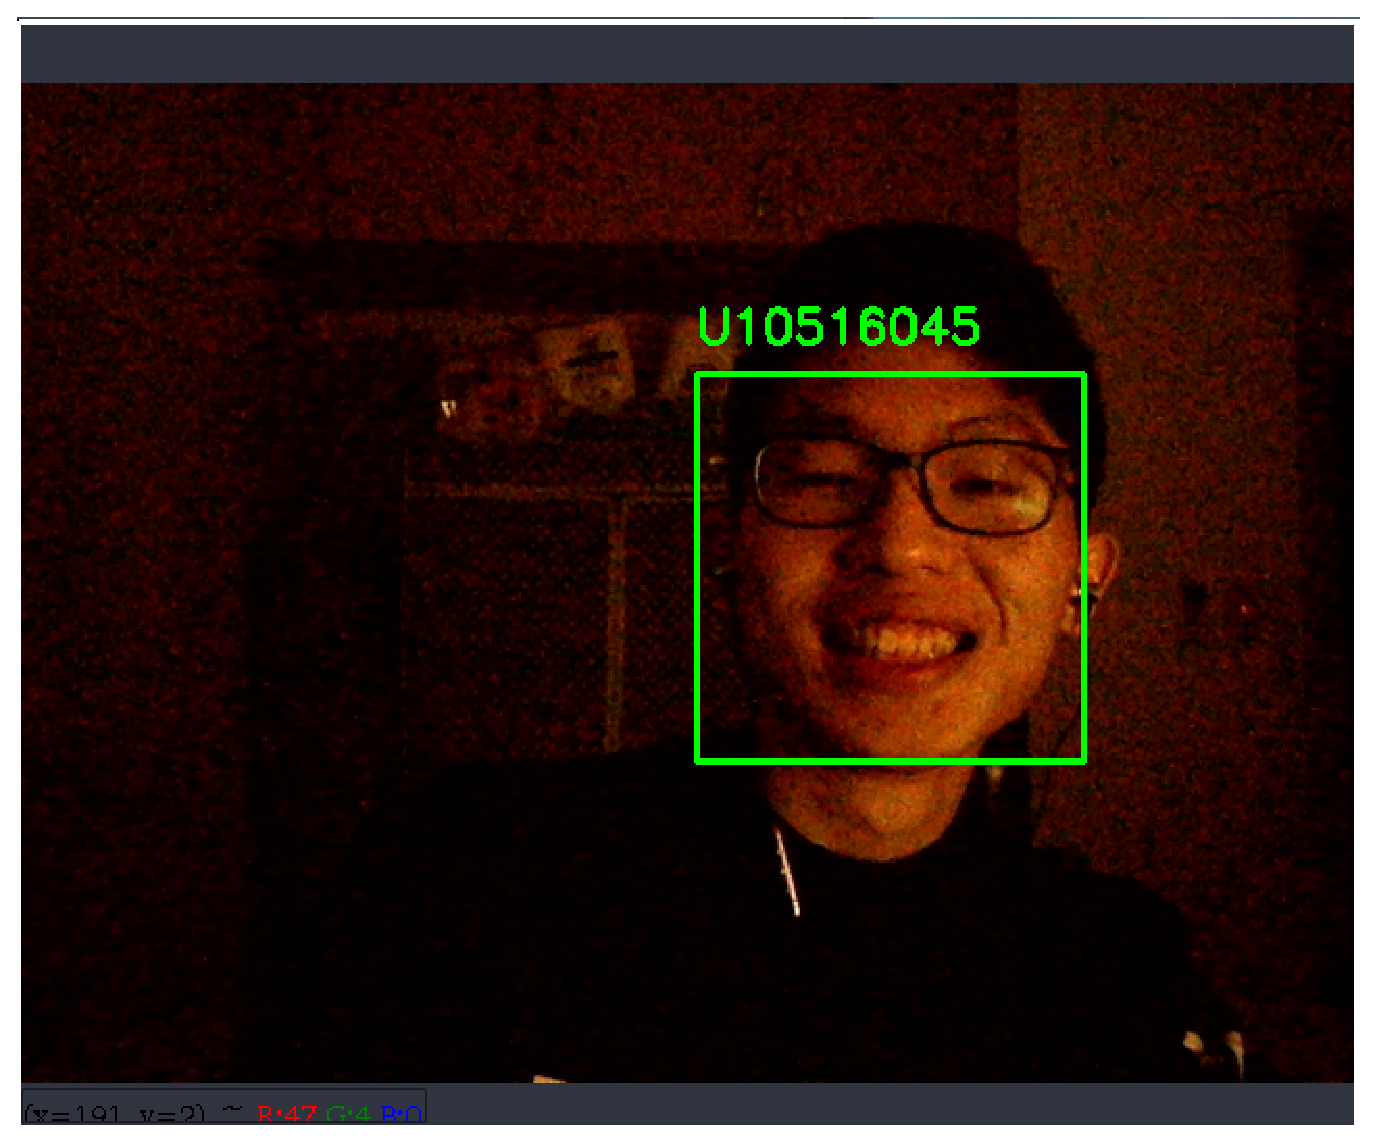
\includegraphics[width=\linewidth]{figures/exp45.eps}
    \caption{U10516045 Guan-Zhong Wang.}
  \end{subfigure}
  \caption{Experimental Result.}
  \label{fig:coffee}
\end{figure}


\section{Discussion}
Since this system is merely a prototype, it still leaves a lot to be desired. For example, I have
not confirmed how many photos must be provided per person in order to make the system recognize each person
correctly. Too few photos will lead to false facial recognition.
\newline

There might also be some alternative approaches that can improve the accuracy of facial recognition. These
issue can be carried on in subsequent studies.


\section{References}
[1] tutorial on pyimagesearch.com (https://www.pyimagesearch.com/2018/06/18/face-recognition-with-opencv-python-and-deep-learning/) by Adrian Rosebrock.\newline\newline
[2] Kaiming He, Xiangyu Zhang, Shaoqing Ren and Jian Sun, "Deep Residual Learning for Image Recognition", 2015 (https://arxiv.org/abs/1512.03385)

\end{document}
